\documentclass[tikz,border=2pt]{standalone}
\usetikzlibrary{arrows.meta}

\begin{document}
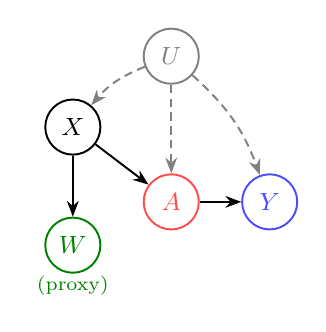
\begin{tikzpicture}[font=\small,
  >={Stealth[length=2mm]},
  var/.style={draw, circle, minimum size=7mm, inner sep=0pt, line width=0.7pt},
  arr/.style={->, line width=0.7pt},
  lat/.style={->, line width=0.7pt, draw=gray, densely dashed}]
  \node[var, draw=gray, text=gray] (U) at (1.25,1.85) {$U$};
  \node[var] (X) at (0,0.95) {$X$};
  \node[var, draw=red!70, text=red!70] (A) at (1.25,0) {$A$};
  \node[var, draw=blue!70, text=blue!70] (Y) at (2.50,0) {$Y$};
  \node[var, draw=green!50!black, text=green!50!black,
    label={[font=\scriptsize, text=green!50!black, yshift=1mm]below:{(proxy)}}] (W) at (0,-0.55) {$W$};

  \draw[arr] (X) -- (A);
  \draw[arr] (A) -- (Y);
  \draw[arr] (X) -- (W);
  \draw[lat] (U) to[bend right=14] (X);
  \draw[lat] (U) -- (A);
  \draw[lat] (U) to[bend left=14] (Y);
\end{tikzpicture}
\end{document}
